\section{Background}
\label{sec:proposal_background}
The advent of deep learning has been transformative, marking a
paradigm shift in our approach to artificial intelligence. Prior to
2011-2012, deep learning was largely deemed impractical. This
perception changed dramatically when a team participating in the
ImageNet Large Scale Visual Recognition Challenge (ILSVRC) in 2012
leveraged deep learning to secure a dominating lead, outperforming
the second-place team by 9.8 percentage points—a margin that
highlighted the difference between second and third place of 0.8.

The roots of deep learning extend back to 1943, yet it remained
largely theoretical until recent advancements in hardware made its
practical application feasible. Today, we stand on the shoulders of
giants, benefiting from the perseverance of researchers who continued
to explore this field despite its challenges.

Quantum computing holds similar transformative potential. The
transformer model represents the next evolutionary step in deep
learning, and by laying the groundwork for a quantum transformer, we
can pave the way for future advancements.

\citet{disipio2021dawn} proposed a quantum-enhanced transformer for
sentiment analysis by adapting the multi-head self-attention and
feed-forward layers to the quantum realm while~\citet{li2023quantum}
introduced Gaussian Projected Quantum Self-Attention, which they used
to create a Quantum Self-Attention Neural Network for text
classification. They argued that this method is more suitable for
handling quantum data than the straightforward inner-product
self-attention used in the work by~\citet{disipio2021dawn}. Notably,
in both models, the computation of attention coefficients and outputs
remains within the classical domain.

In terms of performance,~\citet{Cherrat_2024} provided results
supporting the notion that quantum transformers may match the
performance of their classical counterparts while requiring fewer
resources in terms of runtime and parameter count. However, their
approach has faced criticism, particularly regarding the exponential
cost associated with encoding matrices into quantum states.

The field of quantum computing is poised to revolutionise deep
learning, yet the integration of quantum mechanisms within neural
network architectures remains under-explored. This study seeks to
address the problem of how quantum components, specifically
variational quantum circuits, can be effectively incorporated into
transformer models to enhance their learning efficiency and reduce
generalisation errors. Specifically, we seek to enhance the
quantum-enhanced transformer initially proposed
by~\citet{disipio2021dawn}. We hypothesise that a quantum transformer
will require less training time and exhibit improved performance
metrics compared to its classical counterparts.

\section{Aim}
\label{sec:aim}
To develop and validate a quantum transformer model that integrates
variational quantum circuits into its architecture, thereby enhancing
learning efficiency and reducing generalisation errors. This will involve:

\begin{enumerate}
    \setlength{
  \itemsep}{-1ex}
  \item Analysing the current limitations of classical transformer
    models in terms of learning efficiency and generalisation.
  \item Designing a quantum transformer architecture that
    incorporates variational quantum circuits as a core component.
  \item Comparing the performance of the proposed quantum transformer
    with classical models, focusing on training time and performance metrics.
  \item Assessing the feasibility of the quantum transformer in
    practical applications, considering both its computational
    efficiency and the quality of its outputs.
\end{enumerate}

\section{Methodology}
\label{sec:methodology}
\subsection{Data Collection}
\label{subsec:data_collection}

Before diving into our models, it is essential to outline the
datasets employed in this study. We start with a lightweight dataset,
which lays the groundwork for our initial analysis then transition to
a more sophisticated dataset, presenting a richer set of challenges
and opportunities for our models to tackle.

In this project, we will use three well-known text classification
datasets: the IMDb, Amazon Polarity, and Yelp Reviews Polarity
datasets, to explore the performance of our models.

The IMDb dataset consists of 50,000 movie reviews, making it ideal
for natural language processing and text analytics. This dataset is
designed for binary sentiment classification, where each review is
classified as either positive or negative. With 25,000 movie reviews
allocated for training and another 25,000 for testing, this dataset
offers a robust amount of data for sentiment analysis tasks. Our
model will predict the polarity of reviews, aiming to differentiate
between positive and negative sentiments using deep learning or
classification algorithms.

The Amazon Polarity dataset is a collection of product reviews
sourced from Amazon over an 18-year period. The dataset includes
approximately 35 million reviews up to March 2013. Reviews with
ratings of 1 and 2 are labelled as negative (class 1), while reviews
rated 4 and 5 are labelled as positive (class 2), with reviews rated
3 being excluded. The dataset provides 1,800,000 training samples and
200,000 testing samples for each class, making it a large-scale
dataset well-suited for binary classification tasks. The inclusion of
product and user information, ratings, and plaintext reviews enables
us to further explore consumer sentiment through our text transformer.

The Yelp Reviews Polarity dataset is derived from the 2015 Yelp
Dataset Challenge and consists of 1,569,264 samples of review text.
For this polarity classification task, reviews with star ratings of 1
and 2 are labelled as negative, while reviews rated 3 and 4 are
labelled as positive. The dataset provides 280,000 training samples
and 19,000 test samples per polarity class. This dataset provides
another large and diverse set of review data that can be utilised to
refine our text transformer model, further strengthening its ability
to classify sentiment in various domains.

\subsection{Models}
\label{subsec:models}

\subsubsection{Classical Transformer}
\label{subsubsec:classical_vision_transformer}

We will implement a classical transformer based on the standard
architecture as shown in Figure~\ref{fig:vit_architecture}. While the
diagram represents the structure of a vision
transformer, the overall structure of the text transformer will be
similar, with key modifications to accommodate text-based input. We
chose the standard transformer encoder model to serve as the baseline
for our benchmark. The general steps of our text transformer are as follows:

\begin{enumerate}
    \setlength{
  \itemsep}{-1ex}
  \item The input text is tokenised into sequences of words or
    subwords using a pre-trained tokenizer.
  \item Each token is then transformed into embeddings using a
    pre-trained word embedding model such as BERT.
  \item Since the transformer processes the tokens in parallel, it
    does not inherently capture the order of the sequence. To address
    this, positional embeddings are added to the token embeddings to
    encode the sequential information.
  \item The new embeddings, along with an additional special token
    embedding, are passed through the transformer encoder.
  \item The output of the encoder is then processed by a multi-layer
    perceptron (MLP) head, which converts the token representations
    into a class prediction for sentiment analysis.
\end{enumerate}

\begin{figure}[ht]
  \begin{center} \subfloat[Vision Transformer Architecture]{
    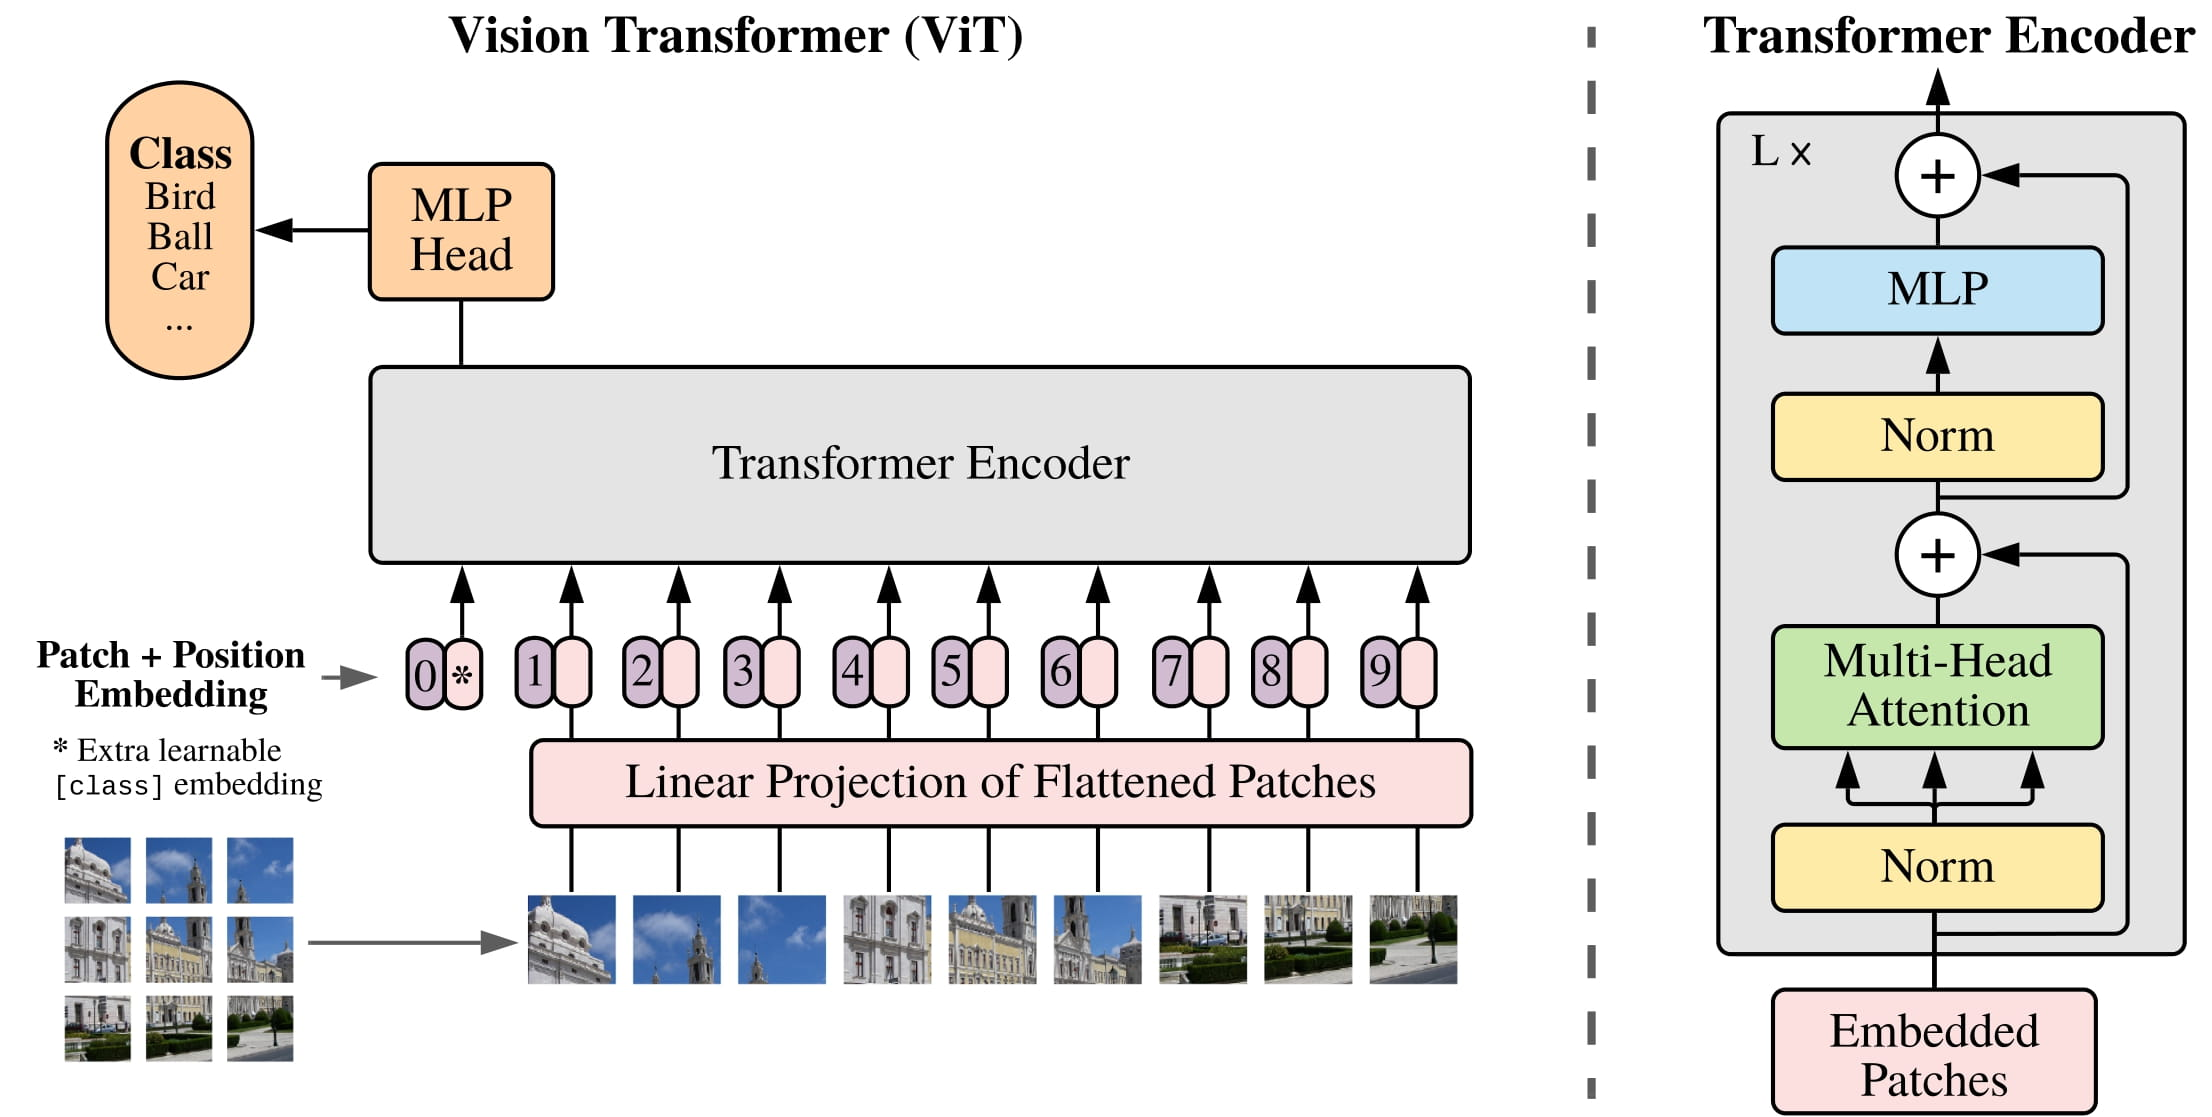
\includegraphics[height=0.4\textwidth]{img/vit_architecture.jpg} }
  \end{center} \vspace{-0.5cm} \caption{An overview of the classical
  model~\cite{dosovitskiy2021image}.}
  \label{fig:vit_architecture}
\end{figure}

In the standard transformer encoder, we use multi-head attention,
which employs several self-attention mechanisms to capture different
types of relationships between tokens. The multi-layer perceptrons
(MLPs) contain two layers with Gaussian Error Linear Unit (GELU)
non-linearity to model complex interactions between tokens. Layer
normalisation stabilises and accelerates training, while residual
connections prevent the vanishing gradient problem.

This architecture will be adapted to text-based sentiment analysis
tasks using datasets such as IMDb, Amazon Polarity, and Yelp Reviews Polarity.

\subsubsection{Quantum Transformer}
\label{subsubsec:quantum_vision_transformer}

\begin{figure}[ht]
  \begin{center}
    \subfloat[Quantum Vision Transformer Architecture]{
      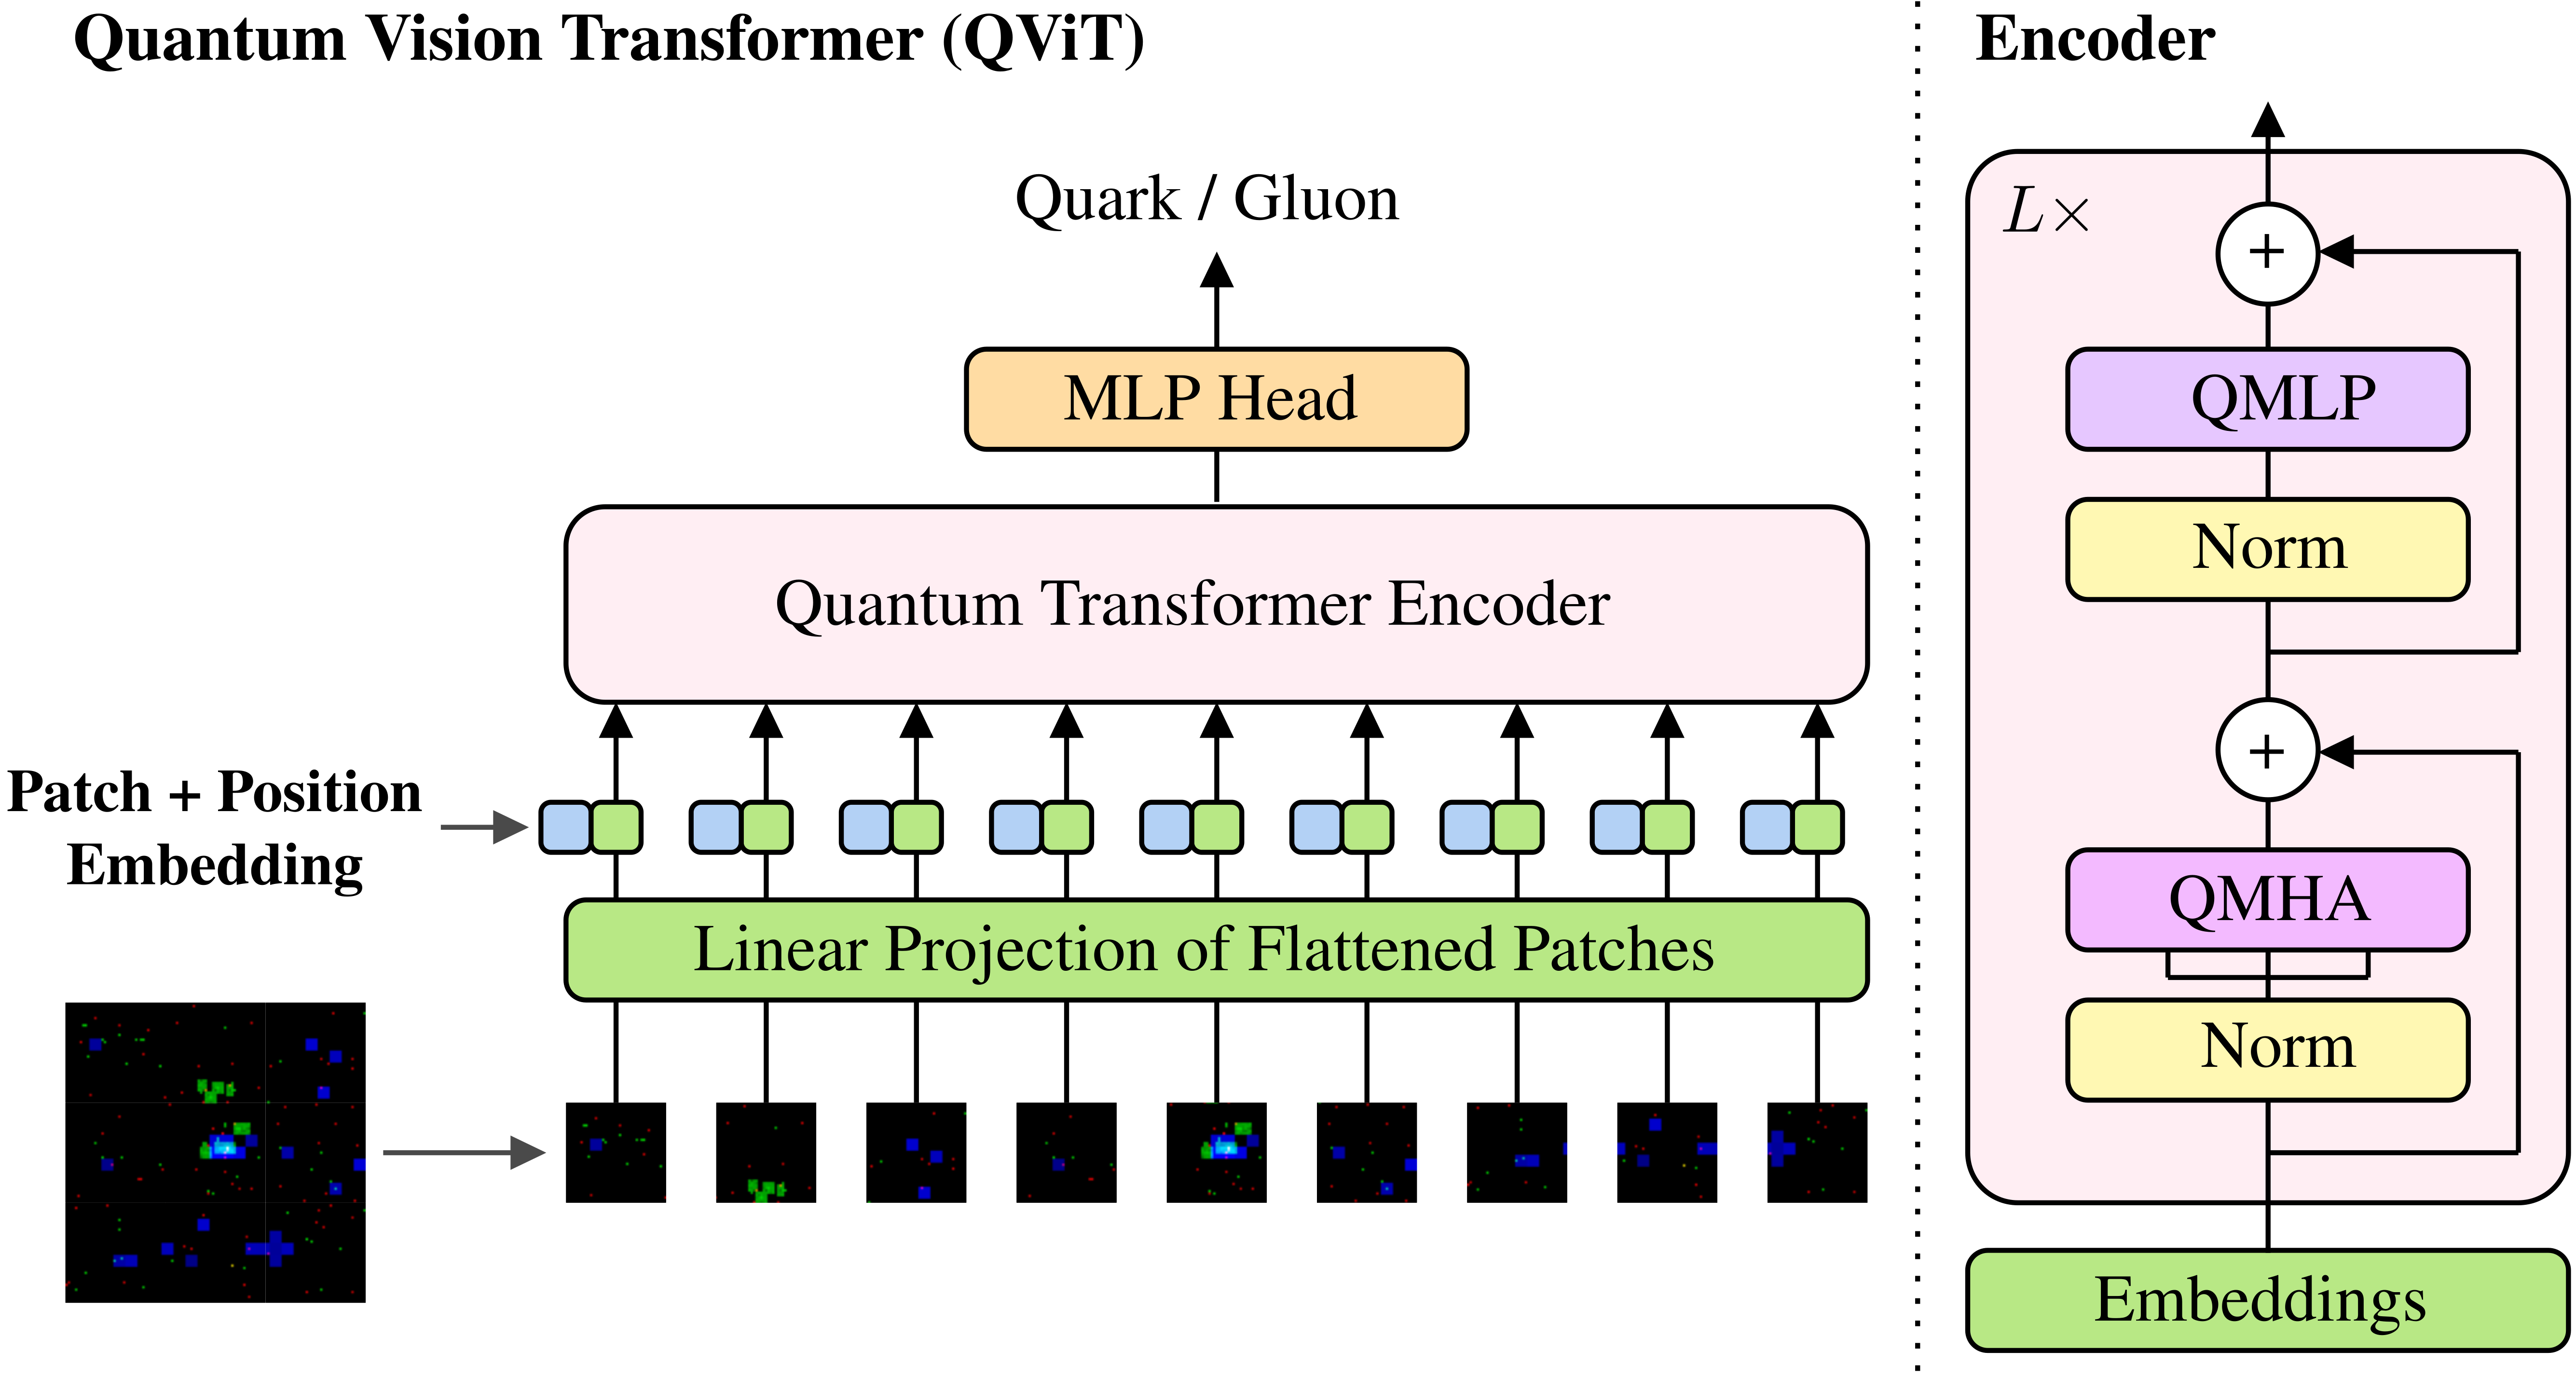
\includegraphics[height=0.4\textwidth]{img/qvit_architecture.png}
    }
  \end{center}
  \vspace{-0.5cm}
  \caption{An overview of the quantum model~\cite{Cara_2023}. The
    illustration of the Transformer Encoder was inspired
  by~\citet{disipio2021dawn}.}
  \label{fig:qvit_architecture}
\end{figure}

\citet{Cara_2023} introduced a model depicted in
Figure~\ref{fig:qvit_architecture}, which incorporates variational
quantum circuits into the multi-head attention and multi-layer
perceptron components of the original architecture. These circuits
serve as the equivalent of fully-connected layers within both
components, potentially offering improved performance in specific
tasks. As our comprehension of the quantum transformer
deepens, the model may be further augmented with additional quantum components.

\subsection{Training and Evaluation}
\label{subsec:training_and_evaluation}

To maintain consistency with the previous work by \citet{Cara_2023}
and \citet{Cherrat_2024}, we will adopt similar hyper-parameters:
cross-entropy loss function, Adam optimizer, 100 training epochs, a
batch size of 32 and a learning rate of \(10^{-3}\).

For model performance evaluation, we will employ two metrics: the
area under the receiver operating characteristic (ROC) curve (AUC)
and accuracy (ACC).

\section{Software and Hardware Requirements}
\label{sec:requirements}

\subsection{Software}
\label{subsec:software}
\begin{itemize}
    \setlength{
  \itemsep}{-1ex}
  \item Python: An easy-to-learn and really popular programming
    language to write quantum code.
  \item PyTorch: A Python library for deep learning.
  \item TensorFlow: Another Python library for deep learning.
  \item PennyLane: A Python library for quantum machine learning.
  \item TensorCircuit: Another Python library for quantum machine learning.
  \item Overleaf: An online latex editor for documentation.
  \item GitHub: An online hub to version control the code for this project.
  \item Visual Studio Code: A code editor to write Python code and
    SSH into Kaya.
  \item Hugging Face: A machine learning platform for sharing machine
    learning models and datasets.
\end{itemize}

\subsection{Hardware}
\label{subsec:hardware}

\begin{itemize}
    \setlength{
  \itemsep}{-1ex}
  \item Personal Laptop: A device to write and edit code.
  \item Kaya: The UWA High-Performance Computational Research Platform.
\end{itemize}

\section{Timeline}
\label{sec:timeline}
The following comprises a rough timeline for the outlined project.

\begin{itemize}
    \setlength{
  \itemsep}{-1ex}
  \item Research proposal: 18th of March
  \item Quantum Computing Study: February - 14 October
    \begin{itemize}
        \setlength{
      \itemsep}{-1ex}
      \item Textbook Readings:
        \begin{itemize}
          \item Explorations in Quantum Computing (Recommended by Jingbo)
          \item Quantum Computing for Computer Scientists
            (Recommended by Microsoft)
          \item Quantum Computation and Quantum Information
            (Recommended in the Quantum Computing Subreddit)
        \end{itemize}
      \item Interactive Learning:
        \begin{itemize}
          \item IBM Quantum
          \item Microsoft Azure Quantum
          \item PennyLane Xanadu Quantum Codebook
        \end{itemize}
    \end{itemize}
  \item Implement a classical transformer from scratch: 18 March - 31 March
  \item Train and evaluate the transformer: April - May
  \item Literature Review: March - 13 May
  \item Implement a quantum transformer: May - August
  \item Seminar Abstract: August - 16 September
  \item Seminar: August - (30 September - 4 October)
  \item Thesis: August - 14 October
\end{itemize}
